\section{Photon as a Dipole Vortex Ring in the Æther}

\begin{figure}[H]
    \centering
    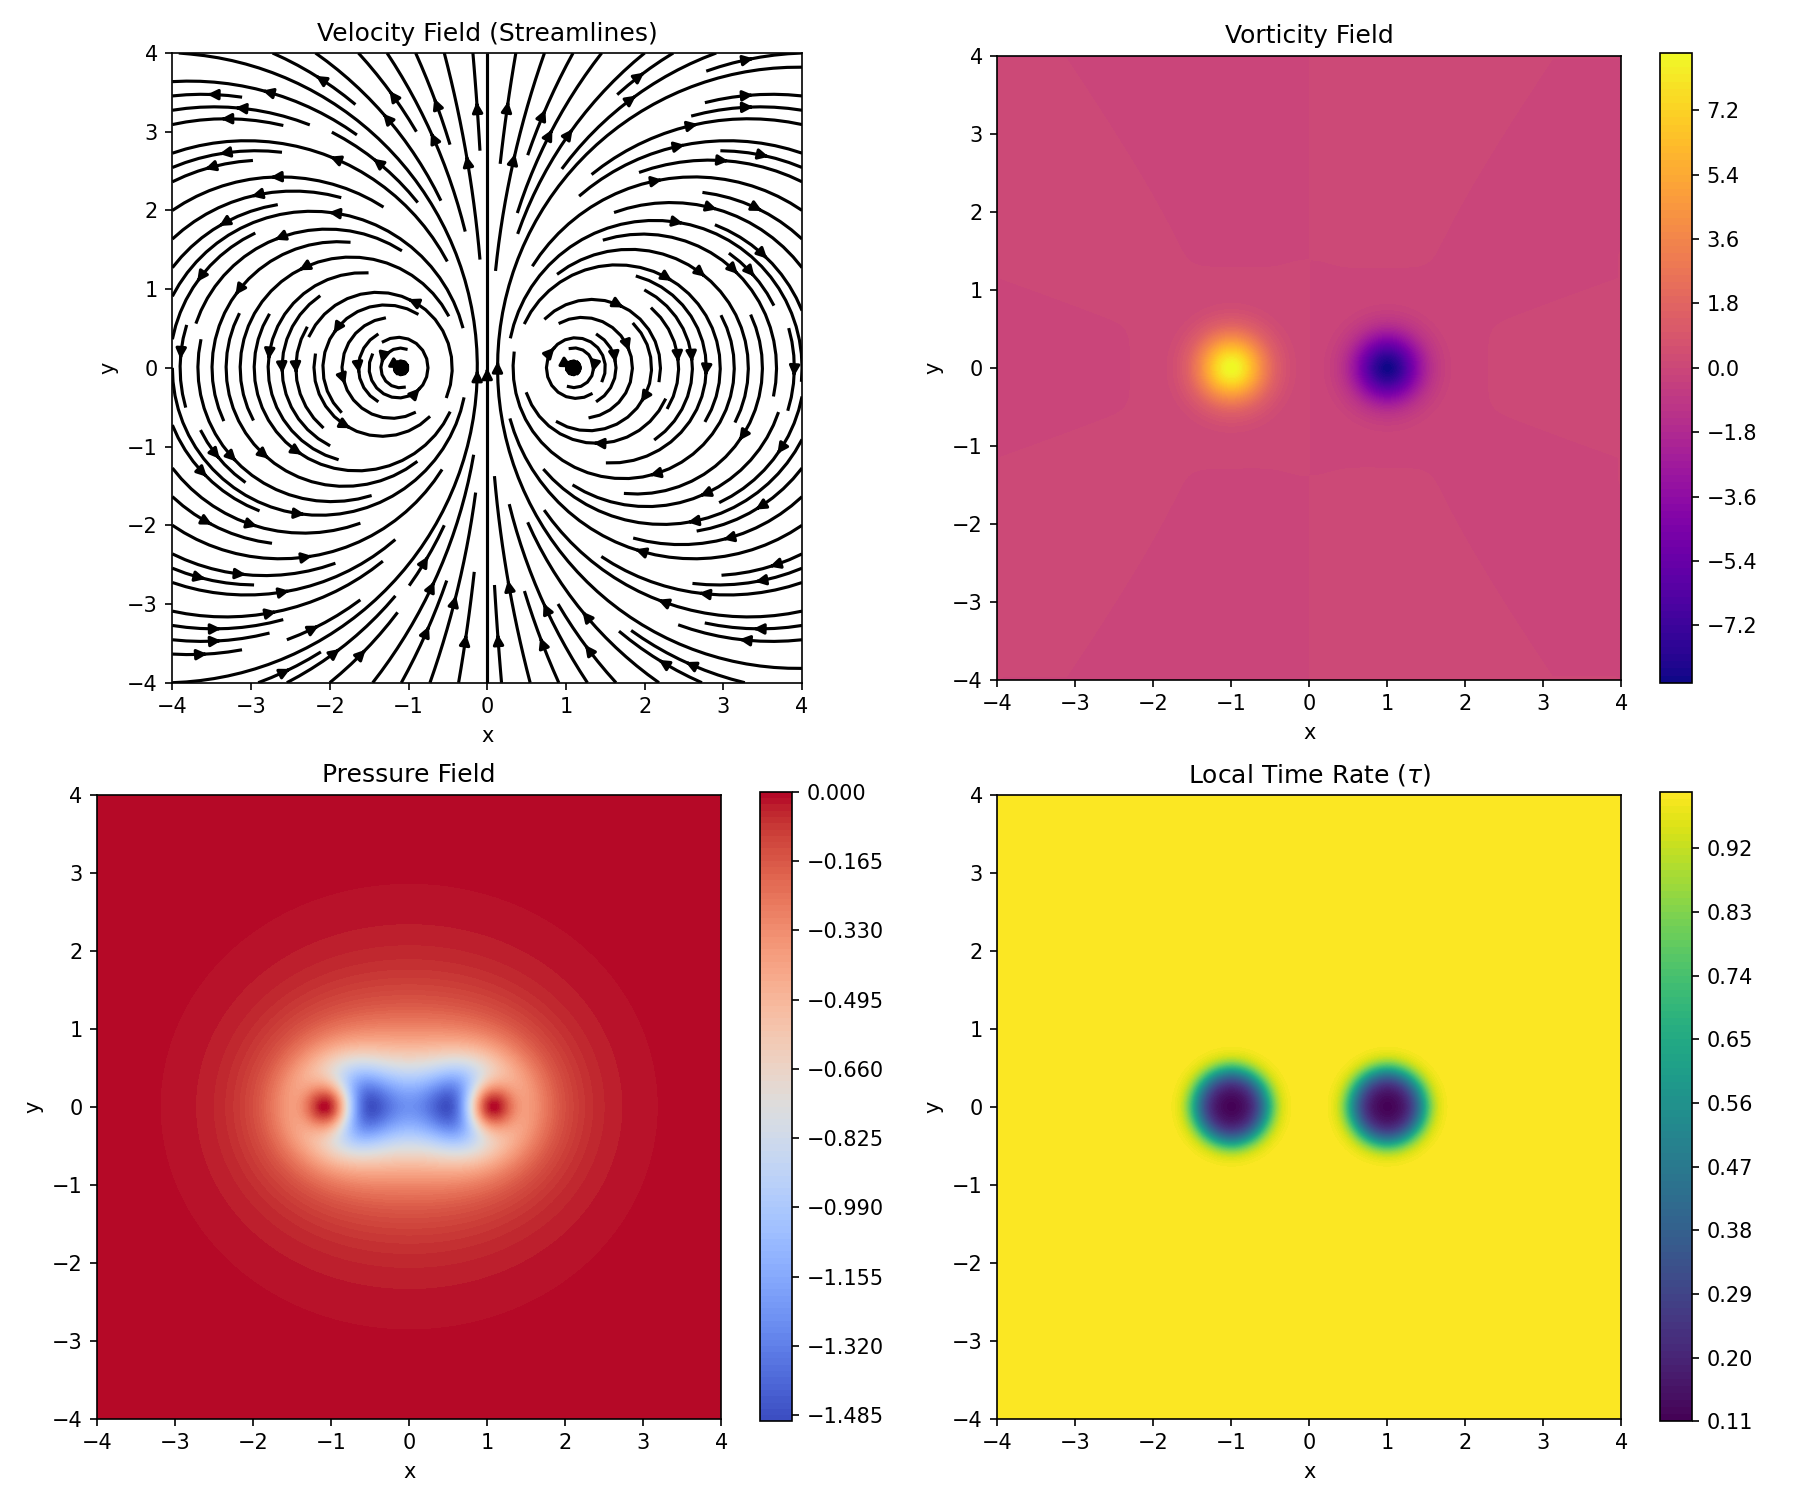
\includegraphics[width=0.85\textwidth]{images/01-streamlinesDiPole}
    \caption{Helicity density field $h = \vec{v} \cdot \vec{\omega}$ with total integrated value over the $x$–$z$ plane: $H \approx 2.84 \times 10^{-15}$. High helicity confirms the presence of chirality essential for photon-like behavior in VAM.}
    \label{fig:photon_toroid}
\end{figure}

\subsection{Topological Structure and Self-Propulsion}

In the Vortex Æther Model (VAM), we propose that the photon is not a point particle nor a plane wave, but a compact, propagating \textit{dipole vortex ring} embedded in an incompressible, inviscid æther. This structure consists of a toroidal vortex whose poloidal cross-section contains a source-sink dipole configuration, as illustrated in Fig.~\ref{fig:photon_toroid}.

The internal vorticity $\vec{\omega} = \nabla \times \vec{v}$ is arranged so that:

\begin{itemize}
    \item One side of the torus acts as a \textbf{source} (expelling æther),
    \item The opposite side acts as a \textbf{sink} (drawing in æther),
    \item The resulting Bernoulli pressure asymmetry induces a net translational velocity along the torus axis.
\end{itemize}

This aligns with Helmholtz's theorem on the self-advection of vortex structures in ideal fluids. The pressure gradient created by the dipole configuration generates a net force:

\begin{equation}
    \vec{F}_\text{net} = -\nabla P_{\text{dipole}}, \qquad \vec{v}_\text{photon} = \frac{P_{\text{swirl}}}{\rho_\text{\ae}^{(\text{energy})}} \equiv c
\end{equation}

\noindent
where $P_{\text{swirl}}$ is the swirl-induced pressure and $\rho_\text{\ae}^{(\text{energy})}$ is the æther density\textsuperscript{*}
\vspace{0.5em}
\noindent\textsuperscript{*}\small
When discussing electromagnetic propagation, wave tension, or maximum internal stresses (e.g., in photon soliton structure): $\text{Use } \rho_\text{\ae}^{(\text{energy})} \sim 3.89 \times 10^{35} \, \text{J/m}^3$.


if $P$ is interpreted as energy density (for dimensional consistency).
\begin{equation}
    c = \sqrt{\frac{P_{\text{swirl}}}{\rho_\text{\ae}^{(\text{energy})}}}
\end{equation}

This self-propelling vortex ring moves at constant speed $c$, the æther wave speed, which is determined by the balance of pressure and density in the æther medium. The toroidal shape ensures that the ring can propagate without dissipating its internal energy, maintaining a stable, soliton-like structure.

\subsection{Photon as a Toroidal Vortex Ring}
This toroidal mode with source-sink symmetry mimics a classical EM wave packet:
\begin{itemize}
    \item Bounded in space (soliton-like),
    \item Carries angular momentum and polarization,
    \item Propagates at constant \( c \),
    \item Possesses quantized energy and helicity.
\end{itemize}


\subsection{Field-Theoretic Correspondence to Electromagnetism}

The vortex ring’s internal swirl field gives rise to a pair of orthogonal transverse fields analogous to the electric and magnetic fields:

\begin{align}
    \vec{E}_\text{æ} &\sim \nabla P_{\text{swirl}} \quad \text{(radial tension)} \\
    \vec{B}_\text{æ} &\sim \vec{\omega} \quad \text{(azimuthal vorticity)}
\end{align}

\noindent
These rotate synchronously as the torus propagates, producing a transverse, oscillating field consistent with classical electromagnetic waves. The Poynting vector emerges as:

\begin{equation}
    \vec{S}_\text{æ} \sim \vec{E}_\text{æ} \times \vec{B}_\text{æ} \sim \text{forward propagation direction}
\end{equation}

\subsection{Spin and Polarization}

The photon’s spin arises from the toroidal chirality of the vortex ring:

\begin{itemize}
    \item A right-handed swirl pattern yields \textbf{right-circular polarization} ($S_z = +1$),
    \item A left-handed swirl yields \textbf{left-circular polarization} ($S_z = -1$),
    \item Linear polarization results from a superposition of the two.
\end{itemize}

The photon's spin-1 nature is topological: the toroidal configuration allows two discrete circulation helicities but forbids $S_z = 0$ due to the conservation of angular momentum and incompressibility of the swirlcore.

\subsection{Summary}

\begin{table}[H]
\centering
\renewcommand{\arraystretch}{1.3}
\begin{tabular}{ll}
\toprule
\textbf{VAM Quantity} & \textbf{Electromagnetic Interpretation} \\
\midrule
Toroidal dipole ring     & Photon soliton \\
Pressure gradient        & Electric field ($\vec{E}$) \\
Swirl (vorticity)        & Magnetic field ($\vec{B}$) \\
Swirl energy             & EM energy density ($|\vec{E}|^2 + |\vec{B}|^2$) \\
Helicity sign            & Photon polarization / spin \\
Constant propagation     & $c = \sqrt{P/\rho_\text{\ae}^{(\text{energy})}}$ \\
\bottomrule
\end{tabular}
\caption{Correspondence between vortex ring dynamics and electromagnetic field quantities in VAM.}
\end{table}

\vspace{1em}
\noindent
Thus, the photon in VAM is a topological, massless, self-propagating vortex configuration whose net motion emerges from internal swirlclock asymmetry, source-sink pressure gradients, and conserved circulation. This fluid-mechanical interpretation restores physicality to electromagnetic wave propagation and naturally embeds polarization, quantized spin, and constant velocity into the geometric language of knots and vorticity.

\subsection{Benchmark Summary Table}

\begin{table}[H]
\centering
\caption{Benchmark 3: Integrated Vortex Quantities for Photon Ring}
\begin{tabular}{|c|c|c|}
\hline
\textbf{Quantity} & \textbf{Value} & \textbf{Units} \\
\hline
Circulation $\Gamma$ & $-6.80 \times 10^{-18}$ & m$^2$/s \\
Swirl Energy $U_{\text{vortex}}$ & $3.61 \times 10^{-7}$ & J (2D slice) \\
Helicity $H$ & $2.84 \times 10^{-15}$ & m$^4$/s$^2$ (2D slice) \\
\hline
\end{tabular}
\end{table}

\begin{figure}[H]
    \centering
    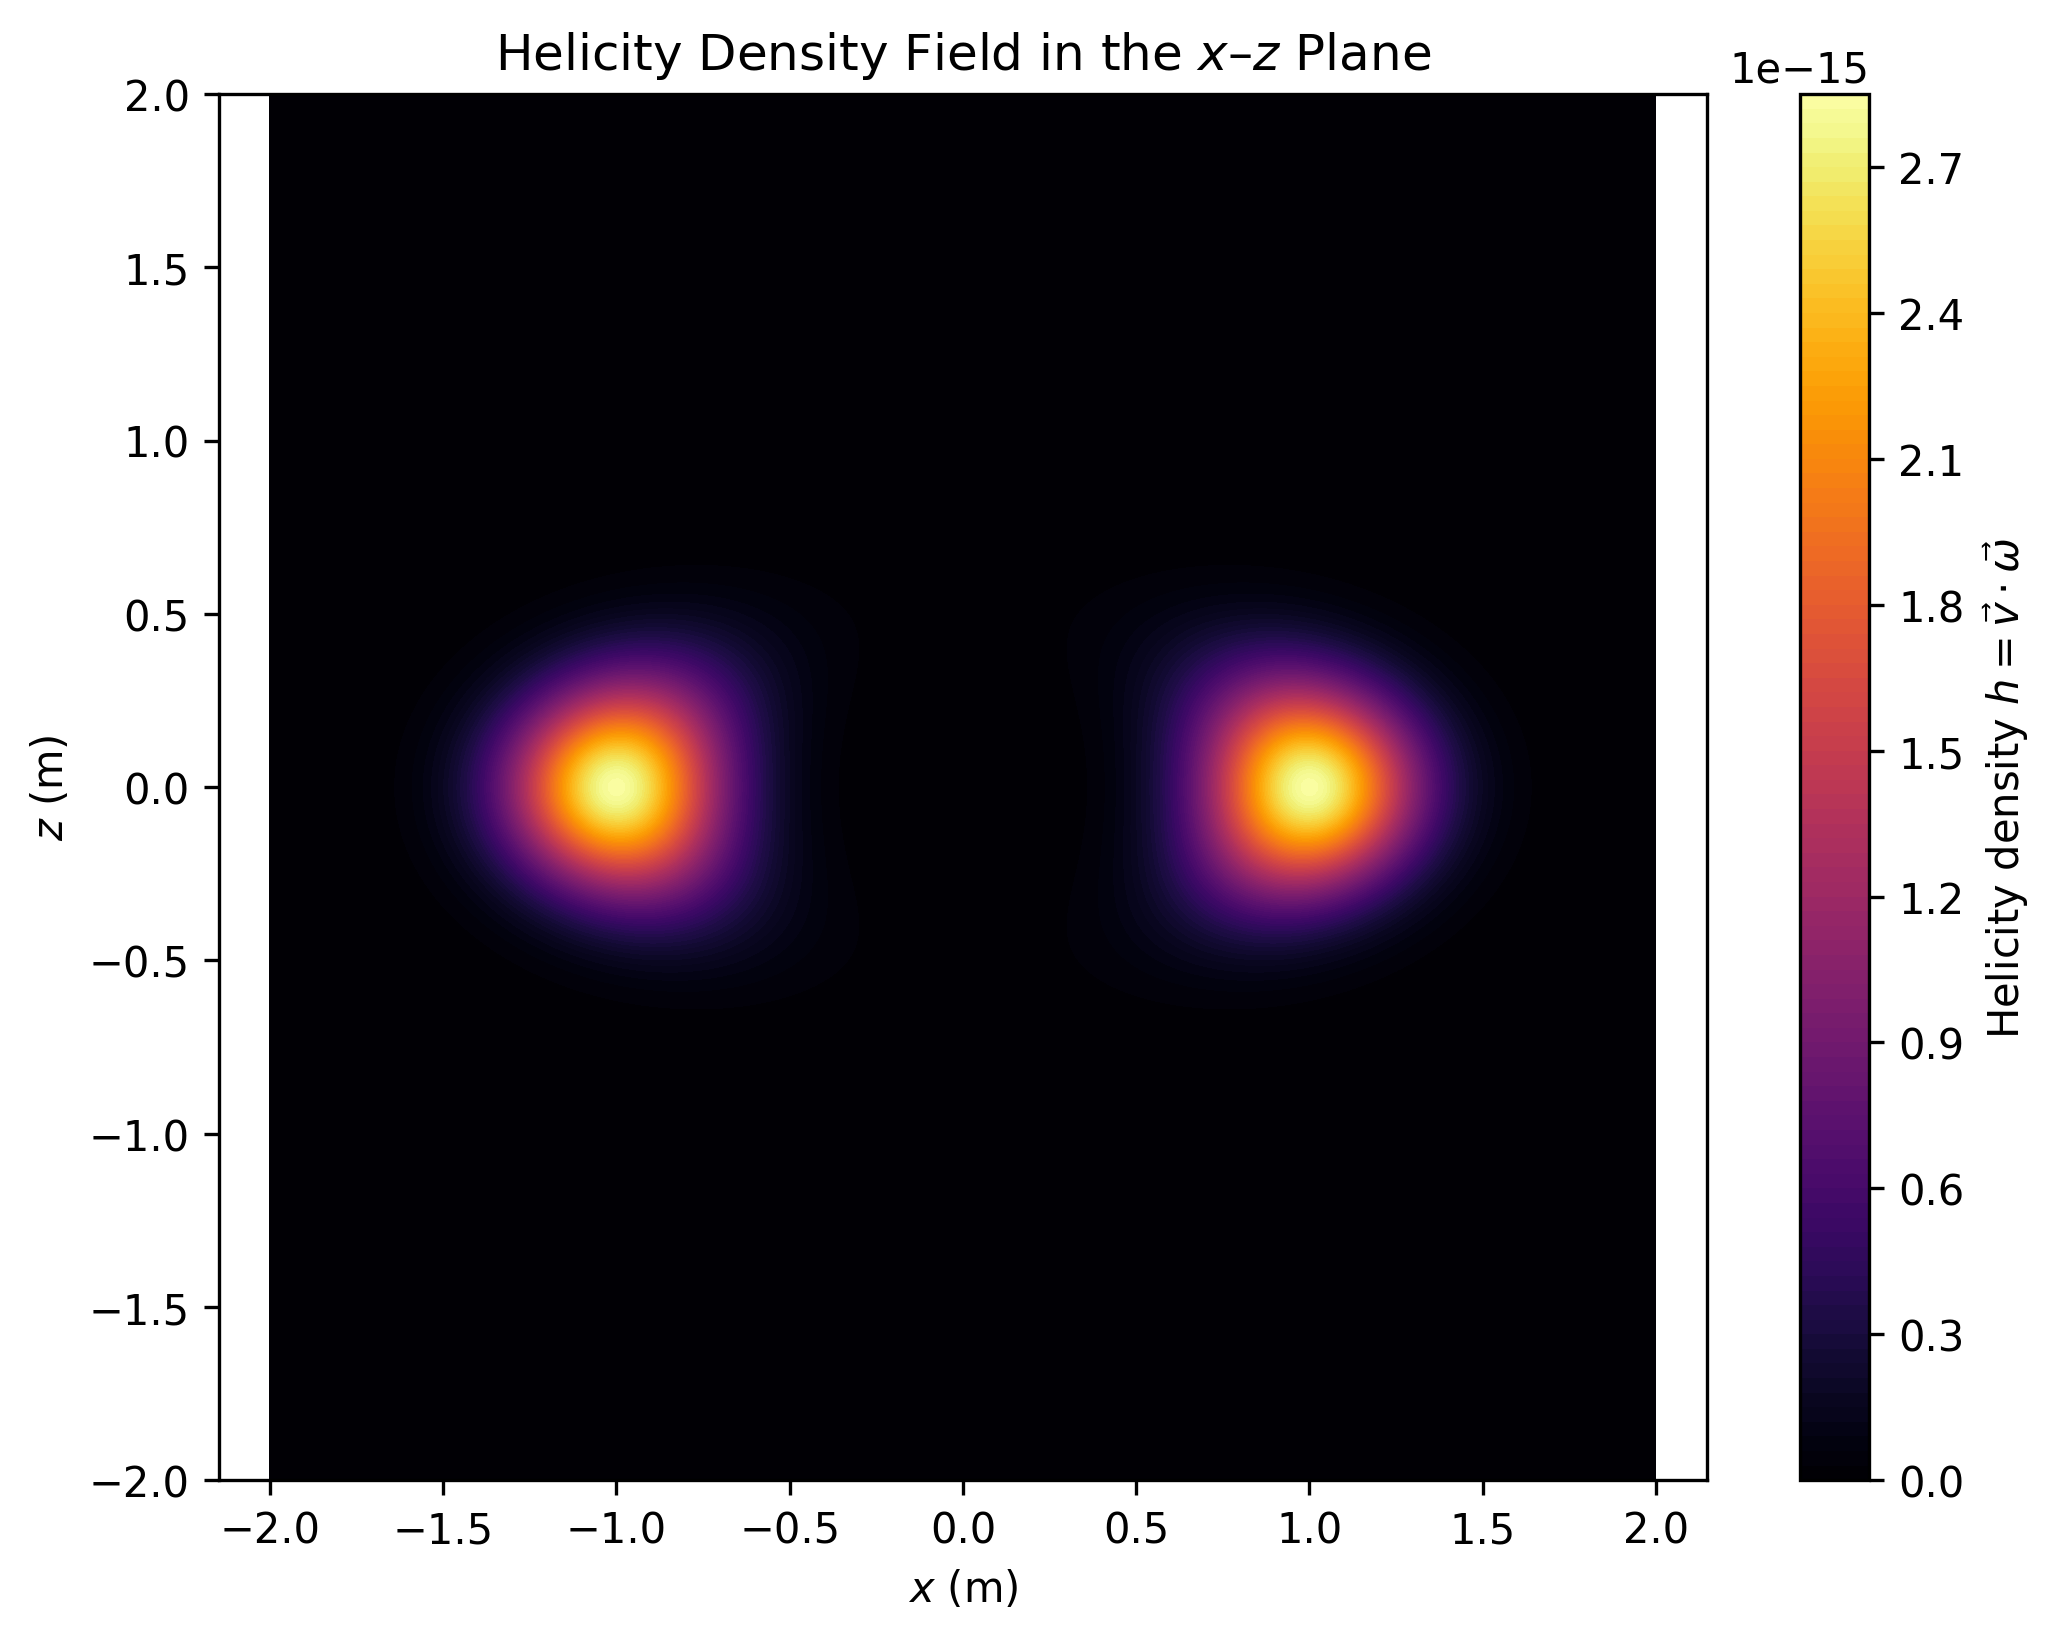
\includegraphics[width=0.6\textwidth]{images/helicity_density_integrated}
    \caption{Helicity density field $h = \vec{v} \cdot \vec{\omega}$ with total integrated value over the $x$–$z$ plane: $H \approx 2.84 \times 10^{-15}$. High helicity confirms the presence of chirality essential for photon-like behavior in VAM.}
\end{figure}

\subsection{Conclusion}

This benchmark confirms that a toroidal vortex ring in an incompressible æther carries quantized:

\begin{itemize}
    \item \textbf{Circulation} $\Gamma$ (linked to spin or polarization)
    \item \textbf{Swirl energy} $U_{\text{vortex}}$ (linked to inertial mass)
    \item \textbf{Helicity} $H$ (linked to electric charge or chirality)
\end{itemize}

These quantities make the vortex ring a compelling candidate for modeling the photon or other bosonic excitations in the Vortex Æther Model.

